\frame{
  \frametitle{Überblick}
%  \tableofcontents[currentsection,hidesubsections,firstsection=12]
  \tableofcontents[firstsection=9]
}

\frame{
  \frametitle{Motivation}

  \begin{itemize}
    \item Datenanalyse erfordert
  \begin{itemize}
    \item Laden/Einlesen von Daten
    \item Transformation, Auswahl, Verknüpfung, \dots
    \item Berechnungen, Statistiken, \dots
    \item \dots
  \end{itemize}
  \item \hl{Welches ist das geeignete Werkzeug?}
  \end{itemize}

  \begin{notebox}
  Maslows Hammer: Wer als Werkzeug nur einen Hammer hat, sieht in jedem Problem einen Nagel.   
  \end{notebox}

  \begin{itemize}
    \item R
    \item \hl{Python + Pandas/scikit-learn/\dots}, \hl{SQL}
    \item Apache Spark/Flink/\dots
  \end{itemize}
  }

    %--------------------------------------------------------------

\frame{
  \frametitle{Motivation /2}

  \begin{itemize}
    \item Datenbanksysteme bieten umfassende Möglichkeiten zur Datenverarbeitung und -analyse
    \begin{itemize}
      \item effiziente Verwaltung (Indexstrukturen, Speicherverwaltung, Fehlersicherheit, Replikation, \dots)
      \item Konsistenzsicherung (Integritätsbedingungen, \dots)
      \item Datenmodellierung
      \item mächtige, deklarative Anfragesprache (SQL)
      \item optimierte Ausführung (Anfrageoptimierung, Parallelisierung, \dots)
    \end{itemize}
    \item \hl{In-Database Analytics} statt Datenexport und/oder dateibasierter Analyse?
  \end{itemize}

  }

  %--------------------------------------------------------------

\frame{
    \frametitle{Datenbank- oder dateibasierte Analyse?}
  
  \begin{columns}[t]
    \begin{column}{0.1\textwidth}
    \hl{Datenbank:}
    \end{column}
    \begin{column}{0.8\textwidth}
      \vspace*{-1.6em}
    \begin{itemize}
      \item Daten bereits in DBMS vorhanden
      \item Daten sind langfristig zu verwalten; werden regelmäßig aktualisiert
      \item wiederholte Analysen
      \item \hl{Import-Aufwand} lohnt sich
    \end{itemize}
  \end{column}
  \end{columns}
  \bigskip
  
  \begin{columns}[t]
    \begin{column}{0.1\textwidth}
    \hl{Dateibasiert:}
  \end{column}
  \begin{column}{0.8\textwidth}
    \vspace*{-1.6em}
      \begin{itemize}
      \item kleinere Datenmengen
      \item schwach strukturierte Daten
      \item nur einmalige Analyse
      \item Analyseverfahren erfordern Datenexport (z.B. Data Mining-Verfahren)
      \item \hl{Import-Aufwand} größer als Analyseaufwand
    \end{itemize}
  \end{column}
  \end{columns}
    }
  

\section{Datenimport mit SQL-DBMS}

\begin{frame}

\frametitle{Laden}

\begin{itemize}
\item Aufgabe
\begin{itemize}
\item Effizientes Einbringen von externen Daten in DBS
\end{itemize}
\item Kritischer Punkt
\begin{itemize}
\item Ladevorgänge blockieren unter Umständen Teile des DBS
\end{itemize}
\item Aspekte
\begin{itemize}
\item Trigger
\item Integritätsbedingungen
\item Indexaktualisierung
\item Update oder Insert?
\end{itemize}
\end{itemize}

\end{frame}

%--------------------------------------------------------------

\begin{frame}

\frametitle{Satzbasiert}

\begin{itemize}
\item Benutzung von Standard-Schnittstellen: \\JDBC, ODBC, \dots
\item Arbeitet im normalen Transaktionskontext
\item Trigger, Indexe und Constraints bleiben aktiv
\begin{itemize}
\item Manuelle Deaktivierung möglich
\end{itemize}
\item Keine großräumigen Sperren
\item Sperren können durch \op{COMMIT} verringert werden
\begin{itemize}
\item Nicht bei DBMS mit MVCC: Leseoperationen werden nie gesperrt 
\end{itemize}
\item Benutzung von Prepared Statements
\item Teilweise proprietäre Erweiterungen (Arrays) verfügbar
\end{itemize}

\end{frame}

%--------------------------------------------------------------

\begin{frame}

    \frametitle{DB-Import am Beispiel von PostgreSQL}
    
    \begin{itemize}
      \item proprietäres SQL-Kommando zum Kopieren von Daten  Tabelle $\leftrightarrow$ Datei
      \item schneller als Folge von Inserts
      \item Formate: Text, CSV, binär
      \item Unterstützung von Header, Trennzeichen, Quotes
      \item Datei muss vom DB-Server lokal erreichbar sein 
      \item Beispiel: Import einer CSV-Datei mit Header
    \end{itemize}

    \begin{sql}    
    COPY movies(title, year) \\
    \1 FROM '/data/movies.csv' \\
    \1 DELIMITER ',' CSV HEADER;
    \end{sql}
\end{frame}

%--------------------------------------------------------------

\begin{frame}

    \frametitle{Multi-Table-Insert in Oracle}
    
    \begin{itemize}
    \item Einfügen in mehrere Tabellen bzw. mehrfach (z.B. für Pivoting)
    
    \hspace*{-1cm}\begin{sql}
    \op{INSERT ALL} \\
    \op{INTO} Quartal\_Verkauf \\
    \1 \op{VALUES} (Produkt\_Nr, Jahr || '/Q1', Umsatz\_Q1) \\
    \op{INTO} Quartal\_Verkauf \\
    \1 \op{VALUES} (Produkt\_Nr, Jahr || '/Q2', Umsatz\_Q2) \\
    \op{INTO} Quartal\_Verkauf \\
    \1 \op{VALUES} (Produkt\_Nr, Jahr || '/Q3', Umsatz\_Q3) \\
    \op{INTO} Quartal\_Verkauf \\
    \1 \op{VALUES} (Produkt\_Nr, Jahr || '/Q4', Umsatz\_Q4) \\
    \op{SELECT} \dots\ \op{FROM} \dots
    \end{sql}
    \end{itemize}
    
    \end{frame}
    
    %--------------------------------------------------------------
    
    \begin{frame}
    
    \frametitle{Multi-Table-Insert in Oracle /2}
    
    \begin{itemize}
    \item Bedingtes Einfügen
    
    \hspace*{-1cm}\begin{sql}
    \op{INSERT ALL} \\
    \op{WHEN} ProdNr \op{IN} \\
    \1 (\op{SELECT} ProdNr \op{FROM} Werbe\_Aktionen) \\
    \op{INTO} Aktions\_Verkauf \\
    \1 \op{VALUES} (ProdNr, Quartal, Umsatz) \\
    \op{WHEN} Umsatz > 1000 \\
    \1 \op{INTO} Top\_Produkte \op{VALUES} (ProdNr) \\
    \op{SELECT} \dots\ \op{FROM} \dots
    \end{sql}
    
    \end{itemize}
    
    \end{frame}
    
    %--------------------------------------------------------------
    
    \begin{frame}
    
    \frametitle{Merge in SQL}
    
    \begin{itemize}
    \item Merge: Versuch eines Inserts, bei Fehler (durch Verletzung einer
      Schlüsselbedingung) $\rightarrow$ Update
    \hspace*{-1cm}\begin{sql}
    \op{MERGE INTO} Kunden K \op{USING} Neukunden N \\
    \op{ON} (N.Name = K.Name \op{AND} N.GebDatum = K.GebDatum) \\
    \op{WHEN MATCHED THEN} \\
    \op{UPDATE SET} K.Name = N.Name, K.Vorname=N.Vorname, \\
    \1 K.GebDatum=N.GebDatum \\
    \op{WHEN NOT MATCHED THEN} \\
    \op{INSERT VALUES} (MySeq.NextVal, N.Name, \\
    \1 N.Vorname, N.GebDatum)
    \end{sql}
    
    \end{itemize}
    
    \end{frame}

    %--------------------------------------------------------------
    
\section{Datenanalyse mit SQL}

\begin{frame}
    \frametitle{Gruppierung und Aggregation}
    
    \begin{itemize}
    \item Datenanalyse: Aggregation mehrdimensionaler Daten
    \item Aggregatfunktion: "`dimensionsfreie"' Antwort
    \begin{itemize}
    \item Standard: \op{SUM}, \op{MIN}, \op{MAX}, \op{COUNT}
    \item Erweiterungen: statistische, physikalische und Finanzfunktionen
    \item Benutzerdefinierte Aggregatfunktionen
    \end{itemize}
    \item Gruppierung: "`1-dimensionale"' Antwort
    \begin{itemize}
    \item Ergebnis: Tabelle mit Aggregatwerten indiziert durch Menge von Attributen
    \end{itemize}
    \end{itemize}
    
    \end{frame}
    
    %---------------------------------------------------------------------
    
    \begin{frame}
    \frametitle{Gruppierung und Aggregation (2)}
    
    \begin{itemize}
    \item SQL: \op{GROUP BY}\emph{ attrib\_liste} [ \op{HAVING} \emph{bedingung} ]
    \begin{itemize}
    \item Gruppierung bzgl. gleicher Werte der Gruppierungsattribute
    \item Abschließende Projektion nur über Gruppierungsattribute oder
      Aggregationen
    \end{itemize}
    \item Einschränkungen
    \begin{itemize}
    \item Berechnung von Histogrammen: Aggregationen über berechnete
      Kategorien\\
    \texttt{... \op{GROUP BY} func(Zeit) \op{AS} Woche ...}
    \item Berechnung von Zwischen- und Gesamtsummen
    \item Berechnung von Kreuztabellen
    \end{itemize}
    \end{itemize}
    
    \end{frame}
    
    %---------------------------------------------------------------------
    \begin{frame}
    \frametitle{Aggregatfunktionen}
    
    \begin{itemize}
    \item Standard-SQL-Funktionen wie \op{MIN}, \op{MAX}, \op{SUM},
      \op{COUNT}, \op{AVG}
    \item neue Funktionen in SQL:2003 für Varianz
      \texttt{\op{VAR\_POP}($x$)}, Standardabweichung \texttt{\op{STDDEV\_POP}($x$)},
      Kovarianz \texttt{\op{COVAR\_POP}($x$, $y$)}  und
      Korrelationskoeffizienten  \texttt{\op{CORR}($x$, $y$)}
    \item jeweils für die gesamte Population (\op{\_POP}) bzw. mit
      Bessel-Korrektur (\op{\_SAMP})
    \end{itemize}
    
    \end{frame}
    
    %---------------------------------------------------------------------
    
    \begin{frame}
    \frametitle{Aggregatfunktionen: Beispiele}
    
    \begin{itemize}
    \item Existiert ein (linearer) Zusammenhang zwischen Anzahl der
      verkauften Produkte und deren Verkaufspreis?
    \end{itemize}
    
    \begin{sql}
    \op{SELECT} \op{COVAR\_POP}(V\_Anzahl, P\_Verkaufspreis) \\
    \op{FROM} Verkauf, Produkt \\
    \op{WHERE} V\_Produkt\_ID = P\_ID
    \end{sql}
    
    \begin{itemize}
    \item Werte nahe Null $\approx$ nicht stärker als statistischer Zufall
    \end{itemize}
    
    \end{frame}
    
    %---------------------------------------------------------------------
    
    \begin{frame}
    \frametitle{Aggregatfunktionen: Beispiele}
    
    \begin{itemize}
    \item Kovarianz gibt keinen Aufschluss über Stärke der Korrelation,
      besser Korrelationskoeffizient
    \end{itemize}
    
    \begin{sql}
    \op{SELECT} \op{CORR}(P\_Verkaufspreis, P\_Einkaufspreis), \\
    \> P\_Produktgruppe \\
    \op{FROM} Verkauf, Produkt \\
    \op{WHERE} V\_Produkt\_ID = P\_ID \\
    \op{GROUP BY} P\_Produktgruppe
    \end{sql}
    
    \begin{itemize}
    \item Werte ab $0{,}5$ deuten auf mittlere bis starke Korrelation
    \end{itemize}
    
    \end{frame}
    
    %---------------------------------------------------------------------
    
    \begin{frame}[shrink]
    \frametitle{Aggregatfunktionen: Beispiele}
    
    \begin{itemize}
    \item Regressionsanalyse für Zusammenhang zwischen Anzahl und
      Verkaufspreis
    \item Berechnung von Geradenanstieg \op{REGR\_SLOPE},
      Regressionskoeffizienten \op{REGR\_R2}, mittleren Preis
      \op{REGR\_AVGX} und mittlere Anzahl \op{REGR\_AVGY}
    \end{itemize}
    
    {\begin{sql}
    \op{SELECT} V\_Kanal, \\
    \1\op{REGR\_SLOPE}(V\_Anzahl, P\_Verkaufspreis) \op{AS}
    Anstieg, \\
     \1\op{REGR\_R2}(V\_Anzahl, P\_Verkaufspreis) \op{AS} Koeff, \\
      \1\op{REGR\_COUNT}(V\_Anzahl, P\_Verkaufspreis) \op{AS} Anzahl, \\
      \1\op{REGR\_AVGX}(V\_Anzahl, P\_Verkaufspreis) \op{AS} MPreis, \\
      \1\op{REGR\_AVGY}(V\_Anzahl, P\_Verkaufspreis) \op{AS} MAnzahl \\
    \op{FROM} Verkauf, Produkt, Zeit \\
    \op{WHERE} V\_Produkt\_ID = P\_ID \op{AND} \\
    V\_Zeit\_ID = Z\_ID \op{AND} \op{YEAR}(Z\_Datum) = 2011 \\
    \op{GROUP BY} V\_Kanal
    \end{sql}}
    
    \end{frame}
    
    %---------------------------------------------------------------------
    
    \begin{frame}
    \frametitle{Berechnung von Zwischen- und Gesamtsummen}
    
    
    {\begin{center}\begin{scriptsize}
    \begin{tabular}{|c|c|l|c|c|c|c|}
    \hline
    \rowcolor{Gray} {PGruppe} & {Jahr} & {Bundesland} & {Umsatz} & {Umsatz} & {Umsatz} & {Umsatz} \\
    \rowcolor{Gray}      &      &        & {PGruppe-} & {PGruppe-} &  {PGruppe} & \\
    \rowcolor{Gray}      &      &        & {Jahr-}  & {Jahr}  &  & \\
    \rowcolor{Gray}      &      &        & {Bundesland} &       &  & \\
    \hline\hline
    {Wein} & {2010} & {Sachsen-Anhalt} & {45}    &       &  & \\
            &      & {Th"uringen} & {43}    &       &  & \\
    \hline
            &      &      &        & {88}   &  & \\
    \hline
            & {2011} & {Sachsen-Anhalt} & {47}    &       &  & \\
    \hline
            &      &      &        & {47}   &  & \\
    \hline
            &      &      &        &       & {135}  & \\
    \hline
    {Bier} & {2011} & {Th{\"u}ringen} & {42}    &       &  & \\
    \hline
            &      &      &        & {42}   &  & \\
    \hline
            &      &      &        &       & {42}  & \\
    \hline
            &      &      &        &       &   & {177}\\
    \hline
    \end{tabular}\end{scriptsize}
    \end{center}}
    %
    %{\scriptsize\begin{center}
    %\begin{tabular}{|c|c|c|c|c|c|}
    %\hline
    %Produkt & Jahr & Region & Verk. & Verk. & Verk. \\
    %      &      &        & Prod.- & Prod. & Prod. \\
    %      &      &        & Jahr-  & Jahr  & \\
    %      &      &        & Region &       & \\
    %\hline\hline
    %Rotwein & 2010 & SANH & 135    &       & \\
    %        &      & THÜR & 120    &       & \\
    %        &      &      &        & 255   & \\
    %        & 2011 & SANH & 140    &       & \\
    %        &      & THÜR & 135    &       & \\
    %        &      &      &        & 275   & \\
    %        &      &      &        &       & 530 \\
    %\hline
    %\end{tabular}
    %\end{center}}
    %% Tabelle
    %
    %{\scriptsize\begin{center}
    %\begin{tabular}{|c|c|c|c|}
    %\hline
    %Produkt & Jahr & Region & Verkäufe \\
    %\hline \hline
    %Rotwein & 2010 & SANH & 135 \\
    %Rotwein & 2010 & THÜR & 120 \\
    %Rotwein & 2010 & \ALLresult & 255 \\
    %Rotwein & 2011 & SANH & 140 \\
    %Rotwein & 2011 & THÜR & 135 \\
    %Rotwein & 2011 & \ALLresult & 275 \\
    %Rotwein & \ALLresult & \ALLresult & 530 \\
    %\hline
    %\end{tabular}
    %\end{center}}
    
    \end{frame}
    
    %---------------------------------------------------------------------
    
    \begin{frame}[shrink=10]
    \frametitle{Berechnung von Zwischen- und Gesamtsummen (2)}
    %
    %\begin{sql}
    %  \op{SELECT} Produkt, \op{NULL}, \op{NULL}, \op{SUM}(Verkäufe)\\
    %  \1	\op{FROM} Verkauf\\
    %  \1	\op{WHERE} Produkt = 'Beaujolais'\\
    %  \1	\op{GROUP BY} Produkt\\
    %  \op{UNION}\\
    %  \op{SELECT} Produkt, Jahr, \op{NULL}, \op{SUM}(Verkäufe)\\
    %  \1	\op{FROM} Verkauf\\
    %  \1	\op{WHERE} Produkt = 'Beaujolais'\\
    %  \1	\op{GROUP BY} Produkt, Jahr\\
    %  \op{UNION}\\
    %  \op{SELECT} Produkt, Jahr, Region, \op{SUM}(Verkäufe)\\
    %  \1	\op{FROM} Verkauf\\
    %  \1	\op{WHERE} Produkt = 'Beaujolais'\\
    %  \1 \op{GROUP BY} Produkt, Jahr, Region
    %\end{sql}
    
    \begin{sql}
    -{}- \ccomment{Zwischensumme (1) "uber alle Produktgr., Jahre und Bundesl"ander} \\
    \op{SELECT} P\_Produktgruppe  \op{AS} PGruppe, \op{YEAR}(Z\_Datum), \\
    \1 O\_Bundesland, \op{SUM}(V\_Anzahl * P\_Verkaufspreis) \op{AS} Umsatz \\
    \op{FROM}  Verkauf, Zeit, Produkt, Ort \\
    \op{WHERE}  V\_Zeit\_ID = Z\_ID \op{AND} V\_Produkt\_ID = P\_ID \op{AND} \\
    \1 V\_Ort\_ID = O\_ID \\
    \op{GROUP BY} P\_Produktgruppe, \op{YEAR} (Z\_Datum), O\_Bundesland \\
      \op{UNION ALL} \\
    -{}- \ccomment{Zwischensumme (2) "uber alle Produktgruppen und  Jahre} \\
    \op{SELECT}  P\_Produktgruppe \op{AS} PGruppe, \op{YEAR} (Z\_Datum), \\
    \1 \op{CAST}(\op{NULL AS VARCHAR(50)}), \\
    \1 \op{SUM}(V\_Anzahl * P\_Verkaufspreis) \op{AS} Umsatz  \\
    \op{FROM}  Verkauf, Zeit, Produkt, Ort \\
    \op{WHERE}  V\_Zeit\_ID = Z\_ID \op{AND} V\_Produkt\_ID = P\_ID \op{AND} \\
    \1 V\_Ort\_ID = O\_ID \\
     \op{GROUP BY} P\_Produktgruppe, \op{YEAR}(Z\_Datum)  \\
      \op{UNION ALL}  \\
    \end{sql}
    
    \end{frame}
    
    
    
    %---------------------------------------------------------------------
    
    \begin{frame}[shrink=10]
    \frametitle{Berechnung von Zwischen- und Gesamtsummen (3)}
    
    \begin{sql}
    -{}- \ccomment{Zwischensumme (3) "uber alle Produktgruppen} \\
    \op{SELECT}  P\_Produktgruppe  \op{AS} PGruppe, \op{CAST}(\op{NULL AS  INT}), \\
    \1 \op{CAST}(\op{NULL AS VARCHAR(50)}), \\
    \1 \op{SUM}(V\_Anzahl * P\_Verkaufspreis) \op{AS} Umsatz  \\
    \op{FROM}  Verkauf, Zeit, Produkt, Ort \\
    \op{WHERE} V\_Zeit\_ID = Z\_ID \op{AND} V\_Produkt\_ID = P\_ID \op{AND} \\
    \1 V\_Ort\_ID = O\_ID \\
    \op{GROUP BY} P\_Produktgruppe  \\
     \op{UNION ALL}  \\
    -{}- \ccomment{Gesamtsumme} \\
    \op{SELECT}  \op{CAST}(\op{NULL AS VARCHAR(50)})  \op{AS} PGruppe, \\
    \1 \op{CAST}(\op{NULL AS INT}), \\
    \1 \op{CAST}(\op{NULL AS VARCHAR(50)}), \\
    \1 \op{SUM}(V\_Anzahl * P\_Verkaufspreis) \op{AS} Umsatz  \\
    \op{FROM}  Verkauf, Zeit, Produkt, Ort \\
    \op{WHERE}  V\_Zeit\_ID = Z\_ID \op{AND} V\_Produkt\_ID = P\_ID \op{AND} \\
    \1 V\_Ort\_ID = O\_ID
     \end{sql}
    
    \end{frame}
    
    %---------------------------------------------------------------------
    
    
    \begin{frame}
    \frametitle{Ausschnitt der Zwischen- und Gesamtsummen}
    
    {\begin{center}
    \begin{tabular}{|l|c|l|r|l}
    \hline
    \rowcolor{Gray} {PGruppe} & {Jahr} &  {O\_Bundesland} &  {Umsatz} \\
    \hline \hline
     {Wein} &  {2010} &  {Sachsen-Anhalt} &  {45} \\
     {Wein} &  {2010} &  {Th"uringen} &  {43} \\
     {Wein} &  {2011} &  {Sachsen-Anhalt} &  {47} \\
     {Bier} &  {2011} &  {Th"uringen} &  {42} \\
    \hline
     {Wein} &  {2010} & $NULL$ &  {88} \\
     {Wein} &  {2011} & $NULL$ &  {47} \\
     {Bier} &  {2011} & $NULL$ &  {42} \\
    \hline
     {Wein} & $NULL$ & $NULL$ &  {135} \\
     {Bier} & $NULL$ & $NULL$ &  {42} \\
    \hline
    $NULL$ & $NULL$ & $NULL$ &  {177} \\
    \hline
    \end{tabular}
    \end{center}}
    
    \end{frame}
    
    %---------------------------------------------------------------------
    
    \begin{frame}
    \frametitle{Nachteile der UNION-Variante}
    
    \begin{itemize}
    \item Hoher Aufwand:
    \begin{itemize}
    \item Berechnung aller Teilsummen für $n$ Gruppierungsattribute
      erfordert $2^n$ Teilanfragen
    \item Eventuelle Verbundoperationen müssen mehrfach wiederholt werden
    \end{itemize}
    \item Aufwendige Formulierung:
    \begin{itemize}
    \item Jedoch eventuell Generierung durch OLAP-Werkzeuge
    \item Einhalten der Struktur
    \end{itemize}
    \end{itemize}
    \end{frame}
    
    %---------------------------------------------------------------------
    
    \begin{frame}
    \frametitle{Berechnung von Kreuztabellen}
    
    \begin{itemize}
    \item Symmetrische Aggregation
    \item Auch Pivot-Tabellen
    \end{itemize}
    
    \begin{center}
    \begin{tabular}{|l||c|c|c|}
    \hline
    \rowcolor{Gray} Verkäufe & 2010 & 2011 & Gesamt \\
    \hline \hline
    Thüringen & 120 & 135 & 255 \\
    \hline
    Sachen-Anhalt & 135 & 140 & 275 \\
    \hline
    Gesamt & 255 & 275 & 530 \\
    \hline
    \end{tabular}
    \end{center}
    
    \end{frame}
    
    %---------------------------------------------------------------------
    
    \begin{frame}
    \frametitle{PIVOT in SQL Server}
    
    \begin{sql}
      \op{SELECT} Jahr, [THÜR] \op{AS} Thüringen, \\
      \1 [SANH] \op{AS} Sachsen-Anhalt \\
      \op{FROM} Verkauf \\
      \op{PIVOT} (\op{SUM}(Verkäufe) \op{FOR} \\
      \1 Region \op{IN} ([THÜR], [SANH]))
    \end{sql}
    
    \begin{center}
    \begin{tabular}{|c|c|c|}
    \hline
    \rowcolor{Gray} Jahr & Thüringen & Sachsen-Anhalt \\
    \hline
    \hline
    2010 & 135 & 120 \\
    \hline
    2011 & 140 & 135 \\
    \hline
    \end{tabular}
    \end{center}
    
    \end{frame}
    
    %---------------------------------------------------------------------
    \begin{frame}
    \frametitle{Cube-Operator}
    \begin{itemize}
    \item "`Kurzform"' für Anfragemuster zur Berechnung von Teil- und
      Gesamtsummen
    \item Generierung aller möglichen Gruppierungskombinationen aus
      gegebener Menge von Gruppierungsattributen
    \item Ergebnis: Tabelle mit aggregierten Werten
    \item Gesamtaggregat:
      $$
      \texttt{NULL}, \texttt{NULL}, ..., \texttt{NULL}, f(*)
      $$
    \item Höherdimensionale Ebenen mit weniger \texttt{NULL}-Werten
    \end{itemize}
    
    \end{frame}
    
    %%%%%%%%%%%%%%%%%%%%%%%%%%%%%%%%%%%%%%%%%%%%%%%%%
    
    \begin{frame}[shrink=10]
    
    \frametitle{Cube-Operator: Beispiel}
    
    \begin{minipage}{5.4cm}
    {\tiny
    \begin{tabular}{|l|c|c|c|}
    \hline
    \rowcolor{Gray} \textbf{PGruppe} & \textbf{Bundesland} & \textbf{Jahr} & \textbf{Umsatz} \\
    \hline\hline
    Wein & Sachsen-Anhalt & 2010 & 45 \\
    \hline
    Wein & Thüringen & 2010 & 43 \\
    \hline
    Wein & Sachsen-Anhalt & 2011 & 47 \\
    \hline
    Bier & Thüringen & 2011 & 42 \\
    \hline
    \end{tabular}}
    \end{minipage}%
    \begin{minipage}{1.4cm}
    
\includegraphics[scale=.46]{fig3/Cube-Pfeil.pdf}
    \end{minipage}%
    \begin{minipage}{4cm}
    {\tiny
    \begin{tabular}{|l|l|l|r|}
    \hline
    \rowcolor{Gray} \textbf{PGruppe} & \textbf{Jahr} & \textbf{Bundesland} & \textbf{Umsatz} \\
    \hline\hline
     {Wein} &  {2010} &  {Sachsen-Anhalt} &  {45} \\
    \hline
     {Wein} &  {2010} &  {Th"uringen} &  {43} \\
    \hline
    \dots & \dots & \dots & \dots \\
    \hline
     {Wein} &  {2010} & {NULL} & {88} \\
    \hline
    {Wein} & {2011} & {NULL} & {47} \\
    \hline
    {Bier} & {2011} & {NULL} & {42} \\
    \hline
    {Wein} & {NULL} & {Sachsen-Anhalt} & {92} \\
    \hline
    {Wein} & {NULL} & {Th"uringen} & {43} \\
    \hline
    {Bier} & {NULL} & {Th"uringen} & {42} \\
    \hline
    {Wein} & {NULL} & {NULL} & {135} \\
    \hline
    {Bier} & {NULL} & {NULL} & {42} \\
    \hline
    {NULL} & {2010} & {Sachsen-Anhalt} & {45} \\
    \hline
    \dots & \dots & \dots & \dots \\
    \hline
    {NULL}& {NULL} & {Sachsen-Anhalt} & {92} \\
    \hline
    {NULL} & {NULL} & {Thüringen} & {85} \\
    \hline
    \dots & \dots & \dots & \dots \\
    \hline
    {NULL} & {2010} & {NULL} & {88} \\
    \hline
    {NULL} & {2011} & {NULL} & {89} \\
    \hline
    {NULL} & {NULL} & {NULL} & {177} \\
    \hline
    \end{tabular}}
    \end{minipage}%
    
    
    \end{frame}
    
    %%%%%%%%%%%%%%%%%%%%%%%%%%%%%%%%%%%%%%%%%%%%%%
    
    \begin{frame}
    
    \frametitle{Cube: Details}
    \begin{itemize}
    \item Kardinalität
      \begin{itemize}
      \item $N$ Attribute mit Kardinalität $C_1, C_2, ..., C_N$
      \item Gesamtkardinalität des \op{CUBE}:
      $$
       \prod_{i=1}^{N}(C_i+1)
      $$
      \end{itemize}
    \item Anzahl der Super-Aggregatwerte
      \begin{itemize}
      \item $N$ Attribute in der \op{SELECT}-Klausel
      \item Super-Aggregate: $2^N-1$
      \end{itemize}
    \end{itemize}
    \end{frame}
    
    %%%%%%%%%%%%%%%%%%%%%%%%%%%%%%%%%%%%%%%%%%%%%%
    
    \begin{frame}
    
    \frametitle{Cube-Operator: SQL-Syntax}
    \begin{itemize}
    \item Implementierung in SQL Server, DB2, Oracle
    \end{itemize}
    
    \begin{sql}
        \textbf{SELECT} P\_Produktgruppe \op{AS} PGruppe,\\
     \1 O\_Bundesland, YEAR(Z\_Datum),\\
     \1 \textbf{SUM}(V\_Anzahl * P\_Verkaufspreis) \op{AS} Umsatz\\
        \textbf{FROM} Verkauf, Zeit, Produkt, Ort\\
        \textbf{WHERE} \dots \\
        \textbf{GROUP BY CUBE}(P\_Produktgruppe, O\_Bundesland, \\
    \1 \op{YEAR}(Z\_Datum))
      \end{sql}
    
    \end{frame}
    
      \begin{frame}
    
        \frametitle{Cube-Operator: SQL-Syntax /2}
        \begin{itemize}
    \item Funktion \op{GROUPING}(Attribut)
      \begin{itemize}
      \item Liefert Wert = 1, wenn über Attribut aggregiert wurde
      \item Liefert Wert = 0, wenn nach Attribut gruppiert wurde
      \end{itemize}
    \item Unterdrückung von Teilsummen, z.B. der Gesamtsumme
    \end{itemize}
    
    \begin{sql}
        ... \textbf{HAVING NOT} (\=
        \textbf{GROUPING}(P\_Produktgruppe) = 1 \textbf{AND}\\
        \1  \textbf{GROUPING}(O\_Bundesland) = 1 \textbf{AND}\\
        \1 \textbf{GROUPING}(YEAR(Z\_Datum)) = 1)
    \end{sql}
    
    \end{frame}
    
    %%%%%%%%%%%%%%%%%%%%%%%%%%%%%%%%%%%%%%%%%%%%%%
    \begin{frame}
    
    \frametitle{Rollup-Operator}
    
    
    \begin{itemize}
    \item \op{CUBE}-Operator: \hl{interdimensional}
      \begin{itemize}
      \item anwendbar für Attribute aus unterschiedlichen Dimensionen
      \item Für Roll-Up oder Drill-Down-Operationen zu aufwendig
      \end{itemize}
    \item \op{ROLLUP}-Operator: \hl{intradimensional}
      \begin{itemize}
      \item Generierung der Attributkombinationen
    $$
    (A_1, ..., A_N), (A_1, ..., A_{N-1}), (A_1, A_2), (A_1), ()
    $$
    für gegebene Attribut\textit{liste} $A_1, ..., A_N$
    \end{itemize}
    \end{itemize}
    
    \end{frame}
    
    
    %%%%%%%%%%%%%%%%%%%%%%%%%%%%%%%%%%%%%%%%%%%%%
    
    \begin{frame}
    
    \frametitle{ROLLUP-Operator: Beispiel (einfach)}
    
    
    \begin{itemize}
    \item Anfrage:
    \end{itemize}
    
    \begin{sql}
    \op{SELECT}  P\_Gruppe, Z\_Tag, Z\_Monat, Z\_Jahr, \\
    \1 \op{SUM}(V\_Anzahl * P\_Verkaufspreis) \op{AS} Umsatz \\
    \op{FROM}  Verkauf, Zeit, Produkt, Ort \\
    \op{WHERE}   V\_Produkt\_ID = P\_ID \op{AND} V\_Ort\_ID = O\_ID \op{AND} \\
    \1   V\_Zeit\_ID = Z\_ID \op{AND} \op{YEAR}(Z\_Datum) = 2011 \op{AND}\\
    \1 P\_Produktgruppe = 'Rotwein' \\
    \op{GROUP BY ROLLUP}(Z\_Jahr, Z\_Monat, Z\_Tag)
    \end{sql}
    
    \vspace*{-1em}
    \begin{itemize}
    \item Auswertung:
      \begin{itemize}
      \item Rollup: \texttt{(Z\_Jahr,Z\_Monat,Z\_Tag),
          (Z\_Jahr,Z\_Monat),(Z\_Jahr),()}
      \end{itemize}
    \end{itemize}
    
    \end{frame}
    
    %%%%%%%%%%%%%%%%%%%%%%%%%%%%%%%%%%%%%%%%%%%%
    
    
    \begin{frame}[shrink=10]
    
    \frametitle{ROLLUP-Operator: Beispiel (einfach)}
    
    \begin{center}
      \begin{tabular}{|l|c|l|l|r|}
        \hline
        \rowcolor{Gray}     {Gruppe} & {Tag} & {Monat} & {Jahr} &
        {Umsatz} \\
        \hline
        \hline
         {Rotwein} &  {1} &  {Januar} &  {2011} & 100 \\
         {Rotwein} &  {2} &  {Januar} &  {2011} & 100 \\
        \dots & \dots & \dots & \dots & \dots \\
         {Rotwein} &  {31} &  {Januar} &  {2011} & 100 \\
         {Rotwein} &  {NULL} &  {Januar} &  {2011} & 2000 \\
         {Rotwein} &  {1} &  {Februar} &  {2011} & 100 \\
         {Rotwein} &  {2} &  {Februar} &  {2011} & 100 \\
        \dots & \dots & \dots & \dots & \dots \\
         {Rotwein} &  {28} &  {Februar} &  {2011} & 100 \\
         {Rotwein} &  {NULL} &  {Februar} &  {2011} & 2000 \\
        \dots & \dots & \dots & \dots & \dots \\
         {Rotwein} &  {NULL} &  {NULL} &  {2011} & 24000 \\
    %    \dots & \dots & \dots & \dots & \dots \\
         {Rotwein} &  {NULL} &  {NULL} &  {NULL} & 24000 \\
        \hline
      \end{tabular}
    \end{center}
    
    
    \end{frame}
    
    %%%%%%%%%%%%%%%%%%%%%%%%%%%%%%%%%%%%%%%%%%%%
    
    \begin{frame}
    
    \frametitle{ROLLUP-Operator: Beispiel (zusammengesetzt)}
    
    
    \begin{itemize}
    \item Anfrage:
    \end{itemize}
    \begin{sql}
    \op{SELECT}  P\_Kategorie, P\_Gruppe, O\_Land, O\_Region\\
    \1 \op{SUM}(V\_Anzahl) \op{AS} Verkäufe \\
    \op{FROM}  Verkauf, Zeit, Produkt, Ort \\
    \op{WHERE}  V\_Zeit\_ID = Z\_ID \op{AND} V\_Produkt\_ID = P\_ID \\
    \1 \op{AND}  V\_Ort\_ID = O\_ID \op{AND} \op{YEAR}(Z\_Datum) = 2011 \\
    \op{GROUP BY ROLLUP}(P\_Kategorie, P\_Gruppe), \\
    \1 \op{ROLLUP}(O\_Land, (O\_Region))
    \end{sql}
    
    \vspace*{-1em}
    \begin{itemize}
    \item Auswertung:
      \begin{itemize}
      \item 1. Rollup: \texttt{(P\_Kategorie,P\_Gruppe),
          (P\_Kategorie),()}
      \item 2. Rollup: \texttt{(O\_Land,O\_Region),(O\_Land),()}
      \item Kreuzprodukt beider Kombination
      \end{itemize}
    \end{itemize}
    
    \end{frame}
    
    %%%%%%%%%%%%%%%%%%%%%%%%%%%%%%%%%%%%%%%%%%%%
    
    
    
    \begin{frame}[shrink=10]
    
    \frametitle{ROLLUP-Operator: Beispiel (zusammengesetzt)}
    
    \begin{center}
      \begin{tabular}{|l|l|l|l|l|}
        \hline
        \rowcolor{Gray}     P\_Kategorie&	P\_Gruppe&	Land	&Region&	Verkäufe\\
        \hline
        \hline
        Wein	&Weißwein&	D&	SANH&	102\\
        Wein	&Rotwein&	D&	SANH&	98\\
        Wein &	NULL&	D&	SANH&	200\\
        ...	&...&	...&	...&	...\\
        Wein	&Weißwein&	D&	NULL&	541\\
        Wein	&Rotwein&	D	&NULL&	326\\
        Wein&	NULL	&D	&NULL&	867\\
        ...	&...&	...&	...&	...\\
        Wein &NULL& D & NULL& 1232\\
        ...	&...&	...&	...&	...\\
        NULL& NULL& D& NULL& 1432\\
        ...	&...&	...&	...&	...\\
        NULL &NULL& NULL& NULL& 3456\\
        \hline
      \end{tabular}
    \end{center}
    
    
    \end{frame}
    
    %%%%%%%%%%%%%%%%%%%%%%%%%%%%%%%%%%%%%%%%%%%%
    \begin{frame}
    
    \frametitle{CUBE- vs. ROLLUP-Operator}
    
    
    \begin{itemize}
    \item CUBE-Operator:
      \begin{itemize}
      \item Generiert alle $2^n$ Kombinationen:
        \begin{itemize}
        \item z.B. für 4 Gruppierungsattribute 16 Kombinationen
        \end{itemize}
      \end{itemize}
    \item ROLLUP-Operator:
      \begin{itemize}
      \item Generiert nur Kombinationen mit Superaggregaten:
        \begin{itemize}
        \item $(f_1, f_2, ..., f_n),$
        \item $ ...$
        \item $(f_1, NULL, ..., NULL),$
        \item $(NULL, NULL, ..., NULL)$
        \end{itemize}
      \item $n+1$ Kombinationen
      \end{itemize}
    \end{itemize}
    
    \end{frame}
    
    %%%%%%%%%%%%%%%%%%%%%%%%%%%%%%%%%%%%%%%%%%%%
    
    \begin{frame}
    
    \frametitle{\op{GROUPING SETS}}
    
    \begin{sql}
        \textbf{GROUP BY} ... \textbf{GROUPING SETS}
        (\textit{gruppierung})
      \end{sql}
    
      \begin{itemize}
    \item Gruppierung:
      \begin{itemize}
      \item Einfache Gruppierungskombination, z.B.: \texttt{(O\_Bundesland,
         O\_Stadt)}
      \item Komplexe Gruppierungsbedingung mit \textbf{\texttt{CUBE}} oder
        \op{ROLLUP}
      \end{itemize}
    \end{itemize}
    
    
    \end{frame}
    
    %%%%%%%%%%%%%%%%%%%%%%%%%%%%%%%%%%%%%%%%%%%%
    
    \begin{frame}
    
    \frametitle{GROUPING SETS: Beispiel}
    
    
    \begin{sql}
        ...\\
        \textbf{GROUP BY}\\
        \1	  \textbf{ROLLUP}(P\_Produktgruppe, P\_Produktkategorie),\hl{(1)}\\
        \1    \textbf{GROUPING SETS}((O\_Stadt), (O\_Bundesland)),\hl{(2)}\\
        \1    \textbf{GROUPING SETS}(		\\
        \2 \textbf{ROLLUP}(Jahr, Quartal, Monat), (Woche))\hl{(3)}
      \end{sql}
    
    \begin{itemize}
    \item Bedeutung
      \begin{itemize}
      \item[\hl{(1)}] entlang der Klassifikationshierarchie
      \item[\hl{(2)}] nur für Städte und Bundesländer
      \item[\hl{(3)}] Nutzung der Parallelhierarchie
        \texttt{(Jahr$\to$Quartal$\to$Monat)} sowie \texttt{(Woche)}
      \end{itemize}
    
    \end{itemize}
    
    
    \end{frame}
    
    
    \begin{frame}
    
      \frametitle{Effekt von GROUPING SETS: Beispieldaten}
    
      \begin{center}
      \begin{tabular}{|l|l|l|r|}
        \hline
      \rowcolor{Gray} \textbf{PGruppe} &  \textbf{Bundesland} & \textbf{Jahr} & \textbf{Umsatz} \\
    \hline\hline
    Bier &	Sachsen-Anhalt &	2010	& 51 \\
    Bier &	Sachsen-Anhalt &	2011 &	46 \\
    Bier &	Thüringen	& 2010	& 49 \\
    Bier &	Thüringen	& 2011	& 47 \\
    Wein &	Sachsen-Anhalt	& 2010	& 45 \\
    Wein &	Sachsen-Anhalt	& 2011 & 	47 \\
    Wein &	Thüringen	& 2010	& 43 \\
    Wein &	Thüringen	& 2011	& 42 \\
    \hline
      \end{tabular}
    \end{center}
    
    \end{frame}
    
    \begin{frame}
    
      \frametitle{Effekt von GROUPING SETS}
    
      Simulation von \op{ROLLUP}
      \begin{sql}
        \op{SELECT} Bundesland, Jahr, \op{SUM}(Umsatz) \op{FROM} Verkauf \\
        \op{GROUP BY GROUPING SETS}( \\
        \1 (PGruppe, Bundesland, Jahr), \\
        \1 (PGruppe, Bundesland), (PGruppe), ());
      \end{sql}
    
      {\small
      \begin{center}
        \begin{tabular}{|l|l|l|r|}
          \hline
        \rowcolor{Gray} \textbf{PGruppe} &  \textbf{Bundesland} & \textbf{Jahr} & \textbf{Umsatz} \\
      \hline\hline
      NULL & NULL & NULL & 323 \\
      Wein	& Thüringen	& 2010 &	43 \\
      Bier &	Thüringen	& 2010 &	49 \\
      Wein &	Thüringen & 	NULL &	43 \\
      Bier &	Thüringen	& NULL	 & 91 \\
      Wein		& NULL & NULL &			135 \\
      \multicolumn{4}{|c|}{\dots} \\
      \hline
        \end{tabular}
      \end{center}}
    
    \end{frame}
    
    \begin{frame}
    
      \frametitle{Effekt von GROUPING SETS /2}
    
    \begin{sql}
      \op{SELECT} Bundesland, Jahr, \op{SUM}(Umsatz) \op{FROM} Verkauf \\
      \op{GROUP BY CUBE}(Bundesland, Jahr)
    \end{sql}
    liefert 9 Tupel: (Thüringen, 2010), (Thüringen, 2011), (Sachsen-Anhalt, 2010), \dots (Thüringen, NULL), (Sachsen-Anhalt, NULL), (NULL, NULL)
    
    \begin{sql}
      \op{SELECT} PGruppe, \op{SUM}(Umsatz) \op{FROM} Verkauf \\
      \op{GROUP BY} PGruppe
    \end{sql}
    
    liefert 2 Tupel: Bier, Wein
    \end{frame}
    
    
    
    
    
    \begin{frame}
    
      \frametitle{Effekt von GROUPING SETS /3}
    
      mehrfache Gruppierung ohne \op{GROUPING SETS}
    
      \begin{sql}
        \op{SELECT} PGruppe, Bundesland, Jahr, \op{SUM}(Umsatz) \\
        \op{FROM} Verkauf \\
        \op{GROUP BY} PGruppe, \op{CUBE}(Bundesland, Jahr)
      \end{sql}
    
      berechnet \hl{Kreuzprodukt} der Gruppierungskombinationen $\leadsto$ $2 \cdot 9 = 18$ Kombinationen
    
    \end{frame}
    
    
    \begin{frame}
    
      \frametitle{Effekt von GROUPING SETS /4}
    
    mit \op{GROUPING SETS}
    
    \begin{sql}
      \op{SELECT} PGruppe, Bundesland, Jahr, \op{SUM}(Umsatz) \\
      \op{FROM} Verkauf \\
      \op{GROUP BY GROUPING SETS}(PGruppe, \\
      \1 \op{CUBE}(Bundesland, Jahr))
    \end{sql}
    
     berechnet \hl{Vereinigung} der Gruppierungskombinationen $\leadsto$ $2 + 9 = 11$ Kombinationen
    \end{frame}
    
    \begin{frame}
    
    \frametitle{SQL:2003 -- Sequenzbasierte Operationen}
    
    \begin{itemize}
    \item Seit SQL:1999 -- Erweiterung um OLAP-Funktionen zur attribut- und
      sequenzbasierten Auswertung
    \item Attribut- und tupelbasierte Aggregation
    \item Umsetzung u.a. in Oracle und DB2
    \item Unterstützte Anfragetypen
      \begin{itemize}
      \item Ratio-To-Total
      \item Laufende Summen (Kumulation)
      \item Gleitender Durchschnitt
      \item Ranking-Analyse
      \end{itemize}
    \end{itemize}
    
    \end{frame}
    
    %%%%%%%%%%%%%%%%%%%%%%%%%%%%%%%%%%%%%%%%%%%%
    
    
    \begin{frame}
    
    \frametitle{OLAP-Funktionen: Syntax}
    
    
    
    \begin{center}
      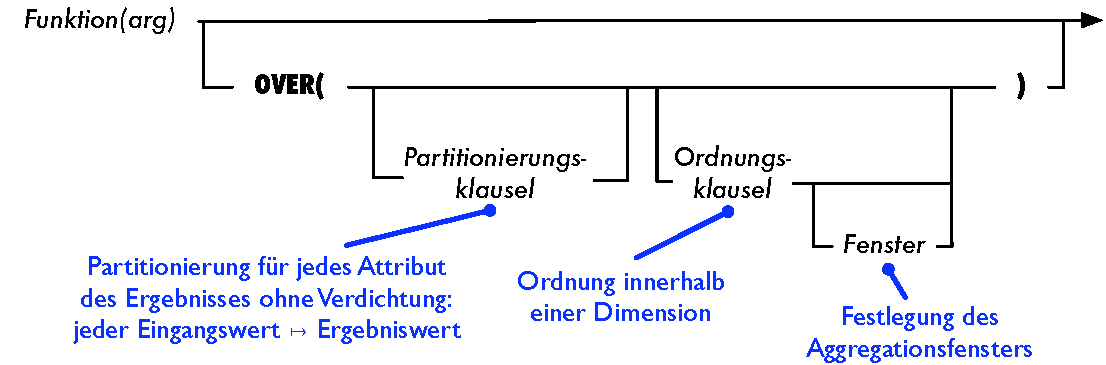
\includegraphics[scale=.6]{fig3/OLAP-Syntax.pdf}
    \end{center}
    
    
    \end{frame}
    
    
    %%%%%%%%%%%%%%%%%%%%%%%%%%%%%%%%%%%%%%%%%%%%
    
    \begin{frame}
    \frametitle{Sichtdefinition für folgende Beispiele}
    
    \begin{sql}
    \op{CREATE VIEW} TagesUmsatz \op{AS} \\
    \1 \op{SELECT} P\_Produktgruppe, Z\_Datum, \\
    \2 \op{SUM}(V\_Anzahl * P\_Verkaufspreis) \op{AS} Umsatz \\
    \1 \op{FROM} Verkauf, Zeit, Produkt \\
    \1 \op{WHERE} V\_Zeit\_Id = Z\_Id \op{AND} V\_Produkt\_Id = P\_Id \\
    \1 \op{GROUP BY} P\_Produktgruppe, Z\_Datum
    \end{sql}
    
    \end{frame}
    
    %%%%%%%%%%%%%%%%%%%%%%%%%%%%%%%%%%%%%%%%%%%%
    
    \begin{frame}
    \frametitle{OLAP-Funktionen: Motivation}
    
    \begin{itemize}
    \item \hl{Ratio-To-Total-Analyse}: Berechnung des Tagesumsatzes am Gesamtumsatz des Monats
      \item Klassische SQL-Anfrage:
    \end{itemize}
    
    \begin{sql}
    \op{SELECT} Z\_Datum, Umsatz,GesamtUmsatz \op{AS} MonatGesamt \\
    \1 100.0*Umsatz/GesamtUmsatz \op{AS} Anteil, \\
    \op{FROM}  TagesUmsatz, \\
    \1 (\op{SELECT} \op{SUM}(Umsatz) \op{AS} GesamtUmsatz \\
    \1 \op{FROM} TagesUmsatz \\
    \1 \op{WHERE} P\_Produktgruppe = 'Wein' \op{AND} \\
    \2 \op{YEAR\_MONTH}(Z\_Datum) = 201108)  Gesamt \\
    \op{WHERE}  P\_Produktgruppe = 'Wein' \op{AND} \\
    \1 \op{YEAR\_MONTH}(Z\_Datum) = 201108
      \end{sql}
    
    \end{frame}
    
    \begin{frame}
      \frametitle{OLAP-Funktionen: Motivation /2}
    
      \begin{itemize}
      \item Innere Unteranfrage berechnet die Gesamtmenge für die
        Anteilsberechnung:
      \end{itemize}
    
      \begin{sql}
          ( \= \op{SELECT} \op{SUM}(Umsatz) \op{AS} GesamtUmsatz \\
        \1 \op{FROM} TagesUmsatz \op{WHERE} \dots )
        \end{sql}
    
        \begin{itemize}
        \item Umständlich, fehleranfällig, ...
        \end{itemize}
    
    \end{frame}
    
    %---------------------------------------------------------------------
    
    \begin{frame}
    
    \frametitle{Formulierung mittels OLAP-Funktion}
    
    \begin{sql}
    \op{SELECT} Z\_Datum, Umsatz, \\
    \1 100.0*Umsatz/\hl{\op{SUM}(Umsatz) \op{OVER}()} \op{AS} Anteil, \\
    \1 \hl{\op{SUM}(Umsatz) \op{OVER}()} \op{AS} MonatGesamt \\
    \op{FROM}  TagesUmsatz \\
    \op{WHERE}  P\_Produktgruppe = 'Wein' \op{AND} \\
    \1 \op{YEAR\_MONTH}(Z\_Datum) = 201108
      \end{sql}
    
      \begin{itemize}
      \item Aggregation über gesamten Eingangsbereich
      \item Partition für Aggregation wird lokal für jeden Eintrag
        generiert
      \end{itemize}
    
    \end{frame}
    
    %%%%%%%%%%%%%%%%%%%%%%%%%%%%%%%%%%%%%%%%%%%%
    \begin{frame}
    
    \frametitle{Ergebnisrelation}
    
    \begin{center}
    {\small
    \begin{tabular}{|l|r|r|r|}
    \hline
    \rowcolor{Gray} Datum & Umsatz & Anteil & MonatGesamt \\
    \hline\hline
    {01-AUG-2011} & {58} & {4,669} & {1242} \\
    {02-AUG-2011} & {52} & {4,186} & {1242} \\
    {03-AUG-2011} & {64} & {5,152}& {1242} \\
    {04-AUG-2011} & {0} & {0,000} & {1242} \\
    \multicolumn{4}{|c|}{\dots} \\
    {31-AUG-2011} & {47} & {3,784} & {1242} \\
    \multicolumn{4}{|c|}{\dots} \\
    \hline
    \end{tabular}}
    \end{center}
    
    \end{frame}
    
    %%%%%%%%%%%%%%%%%%%%%%%%%%%%%%%%%%%%%%%%%%%%
    
    \begin{frame}
    
    \frametitle{Attributlokale Partitionierung}
    
    
    \begin{itemize}
    \item Partitionierung des Eingabestroms einer OLAP-Funktion (ähnlich
      Gruppierung)
    \item \hl{Aber:} Partitionierung erfolgt pro Attribut/Anweisung der
      Aggregrationsoperation
      \begin{itemize}
      \item Ermöglicht Nachgruppierung
      \end{itemize}
    \end{itemize}
    
    \end{frame}
    
    \begin{frame}
    
      \frametitle{Attributlokale Partitionierung /2}
    
    
      \begin{itemize}
    \item Beispiel: Ermittlung der Anteile der Tagesumsätze im
      Vergleich zum Monatsumsatz
    \end{itemize}
         \begin{sql}
    \op{SELECT} P\_Produktgruppe, Z\_Datum, Umsatz,  \\
    \1 100.0*Umsatz/\op{SUM}(Umsatz) \\
    \2 \op{OVER}(\op{PARTITION BY YEAR\_MONTH}(Z\_Datum),\\
    \3  P\_Produktgruppe) \op{AS} MonatAnteil, \\
    \1 \op{SUM}(Umsatz) \\
    \2 \op{OVER}(\op{PARTITION BY YEAR\_MONTH}(Z\_Datum),\\
    \3 P\_Produktgruppe) \op{AS} MonatGesamt \\
    \op{FROM} TagesUmsatz
      \end{sql}
    \end{frame}
    
    %%%%%%%%%%%%%%%%%%%%%%%%%%%%%%%%%%%%%%%%%%%%
    
    
    \begin{frame}
    
    \frametitle{Attributlokale Partitionierung: Details}
    
    \begin{itemize}
    \item Prinzip:
    \end{itemize}
         \begin{sql}
    \textbf{SUM}(Menge) \textbf{OVER}(\textbf{PARTITION BY
          MONTH}(Z\_Datum))
      \end{sql}
      \begin{itemize}
    \item Spezifikationstext hinter \texttt{\textbf{OVER}} heisst \hl{
        Partitionierungsschema}
    \item Keine Konflikte durch unterschiedliche Partitionierungsschemata
      innerhalb einer Anfrage
      \begin{itemize}
      \item Jeweils alle Einträge einer Partition in Berechnung einbezogen
      \end{itemize}
    \end{itemize}
    
    \end{frame}
    
    %%%%%%%%%%%%%%%%%%%%%%%%%%%%%%%%%%%%%%%%%%%%
    
    \begin{frame}
    
    \frametitle{Sequenzorientierte Analyse}
    
    \begin{itemize}
    \item Spezifikation einer attributlokalen Ordnung für Partitionen
    \item Anwendung: laufende Summe, gleitender Durchschnitt, etc.
    \item Beispiel: kumulierte Umsatzzahlen der Weine über Gesamtzeitraum und pro
      Monat
    \end{itemize}
       \begin{sql}
    \op{SELECT} Z\_Datum,  \\
    \1 \op{SUM}(Umsatz) \op{OVER}(\op{ORDER BY} Z\_Datum) \op{AS} SumGesamt,\\
    %\3 \op{ORDER BY} Z\_Datum) \op{AS} SummeGesamt, \\
    \1 \op{SUM}(Umsatz) \op{OVER}(\\
    \3 \op{PARTITION BY YEAR\_MONTH}(Z\_Datum)\\
    \3 \op{ORDER BY} Z\_Datum) \op{AS}
    SumMonat \\
    \op{FROM}  TagesUmsatz\\
    \op{WHERE}  P\_Produktkategorie = 'Wein'
      \end{sql}
    
    
    \end{frame}
    
    %%%%%%%%%%%%%%%%%%%%%%%%%%%%%%%%%%%%%%%%%%%%
    \begin{frame}
    
      \frametitle{Sequenzorientierte Analyse: Prinzip}
    
    \begin{itemize}
    \item Anzahl der Tupel, die in ein Ergebnistupel eingehen entspricht
      Position des Tupels bzgl. gegebener Ordnung
    \item Eingangstupel $t_i$, Ergebnistupel $s_i$
      \begin{center}
        \begin{tabular}{cclcc}
          $t_1$&	$ \longrightarrow $	&$SUM(\{t_1\})$&	$ \longrightarrow $		&	$s_1$\\
          $t_2$	&	$ \longrightarrow $	&$SUM(\{t_1, t_2\})$	&	$ \longrightarrow $	&	$s_2$\\
          $t_3$&	$ \longrightarrow $	&	$SUM(\{t_1 ,t_2 ,t_3\})$&	$ \longrightarrow $	&	$s_3$\\
          &&...&&
        \end{tabular}
      \end{center}
    \item Schrittweise Vergrößerung des Analysefensters
    \end{itemize}
    
    \end{frame}
    
    %%%%%%%%%%%%%%%%%%%%%%%%%%%%%%%%%%%%%%%%%%%%
    
    
    
    \begin{frame}
    
    \frametitle{Nutzung für Ranking-Analysen}
    \begin{itemize}
    \item Funktionen
      \begin{itemize}
      \item \texttt{\textbf{RANK}()}: liefert Rang eines Tupels
        bzgl. vorgegebener Ordnung innerhalb der Partition
        \begin{itemize}
        \item Bei Duplikaten gleicher Rang (mit Lücken)
        \end{itemize}
      \item \texttt{\textbf{DENSE\_RANK}()}: wie \texttt{\textbf{RANK}()},
        jedoch ohne Lücken
      \end{itemize}
    \item Beispiel: Ranking nach Umsatz
    
    \end{itemize}
    \begin{sql}
    \op{SELECT} Z\_Datum, RANK() \\
    \1 \op{OVER}(\op{ORDER BY} Umsatz DESC) \op{AS} Rang \\
    \op{FROM}  TagesUmsatz \\
    \op{WHERE}  P\_Produktgruppe = 'Wein'
    \end{sql}
    
    \end{frame}
    
    %%%%%%%%%%%%%%%%%%%%%%%%%%%%%%%%%%%%%%%%%%%%%%
    
    \begin{frame}
    
    \frametitle{Ranking-Analyse: Beispiel}
    
    \begin{itemize}
    \item Beschränkung von "`Hitlisten"'
    \item Beispiel: Top-3 der Tage mit den höchsten Umsatzzahlen pro Monat
    \item Anfrage:
    \end{itemize}
      \begin{sql}
        \op{SELECT}  P.Z\_Datum, P.TopMonat\\
        \op{FROM}  (\op{SELECT} Z\_Datum, P\_Produktgruppe,\\
    \2 \op{RANK}() \op{OVER}(\\
    \3 \op{PARTITION BY YEAR\_MONTH}(Z\_Datum)\\
        \3 \op{ORDER BY} Umsatz \op{DESC}) \op{AS} TopMonat\\
        \2 \op{FROM} TagesUmsatz)  P\\
        \op{WHERE} P.TopMonat <= 3 \op{AND}\\
    \1 P.P\_Produktgruppe = 'Wein' \\
        \op{ORDER BY} P.TopMonat \op{DESC}
      \end{sql}
    
    \end{frame}
    
    %%%%%%%%%%%%%%%%%%%%%%%%%%%%%%%%%%%%%%%%%%%%%%
    
    \begin{frame}
    
    \frametitle{Bildung dynamischer Fenster}
    \begin{itemize}
    \item Bisher: nur wachsende Fenstergröße für Partition
    \item Jetzt: explizite Angabe des Fensters
      \begin{itemize}
      \item \texttt{\textbf{ROWS}}: Anzahl der Tupel
      \item \texttt{\textbf{RANGE}}: Anzahl der wertmäßig verschiedenen
        Tupel
      \end{itemize}
    \item Anwendung: gleitender Durchschnitt
    \item Ausgehend von definierten Startpunkt bis zum aktuellen Tupel
      \begin{itemize}
      \item \texttt{\textbf{UNBOUNDED PRECEDING}}: erstes Tupel der
        jeweiligen Partition
      \item \texttt{n \textbf{PRECEDING}}: $n$-ter Vorgänger relativ zur
        aktuellen Position
      \item \texttt{\textbf{CURRENT ROW}}: aktuelles Tupel (nur mit
        \texttt{\textbf{RANGE}} und Duplikaten sinnvoll)
      \end{itemize}
    
    \end{itemize}
    
    \end{frame}
    
    %%%%%%%%%%%%%%%%%%%%%%%%%%%%%%%%%%%%%%%%%%%%%%
    
    \begin{frame}
    
    \frametitle{Bildung dynamischer Fenster /2}
    \begin{itemize}
    \item Angabe der unteren und oberen Schranken
    \end{itemize}
      \begin{sql}
        \textbf{BETWEEN} untereGrenze \textbf{AND} obereGrenze
      \end{sql}
      \begin{itemize}
    \item Spezifikation der Grenzen
      \begin{itemize}
      \item \texttt{\textbf{UNBOUNDED PRECEDING}}
      \item \texttt{\textbf{UNBOUNDED FOLLOWING}}
      \item \texttt{n \textbf{PRECEDING}}
      \item \texttt{n \textbf{FOLLOWING}}
      \item \texttt{\textbf{CURRENT ROW}}
      \end{itemize}
    \item \texttt{obereGrenze} muss höhere Position als
      \texttt{untereGrenze} spezifizieren
    \end{itemize}
    
    \end{frame}
    
    %%%%%%%%%%%%%%%%%%%%%%%%%%%%%%%%%%%%%%%%%%%%%%
    \begin{frame}
    
    \frametitle{Dynamische Fenster: Beispiel}
    
    \begin{itemize}
    \item Gleitender Durchschnitt mit 5-Tage-Fenster auf Monatsebene
    \end{itemize}
    
    %\hspace*{-.5cm}
    \begin{sql}
        \op{SELECT}  Z\_Datum, \op{AVG}(Umsatz) \op{OVER}(\\
        \2		\op{PARTITION BY YEAR\_MONTH}(Z\_Datum) \\
        \2		\op{ORDER BY} Z\_Datum \\
        \2		\op{ROWS BETWEEN} 2 \op{PRECEDING} \\
        \2		\op{AND} 2 \op{FOLLOWING}) \op{AS} Durch5Tage\\
        \op{FROM}  TagesUmsatz \\
    \op{WHERE} P\_Produktkategorie = 'Wein'
      \end{sql}
    
    \end{frame}
    
    \begin{frame}
    
      \frametitle{OLAP-Funktionen: Zusammenfassung}
    
    Beispieltabelle \texttt{Numbers}
    
    \begin{center}
      \begin{tabular}{|c|c|}
      \hline
      \rowcolor{Gray} grp & val \\
      \hline \hline
      10 & 1 \\
      10 & 2 \\
      10 & 3 \\
      20 & 4 \\
      20 & 5 \\
      20 & 6 \\
      30 & 7 \\
      30 & 8 \\
      30 & 9 \\
      \hline
      \end{tabular}
      \end{center}
    
    \end{frame}
    
      %----------------------------------
    
    
    \begin{frame}
    
    \frametitle{OLAP-Funktionen: Effekt der \op{OVER}-Klausel}
    
    \begin{sql}
      \op{SELECT} val, \\
      \1 \op{SUM}(val) \op{OVER}() \op{AS} sum1, \\
      \1 \op{SUM}(val) \op{OVER}(\op{ORDER BY} val) \op{AS} sum2 \\
      \op{FROM} Numbers
    \end{sql}
    
    \begin{center}
      \begin{tabular}{|c|c|c|}
      \hline
      \rowcolor{Gray} val & sum1 & sum2 \\
      \hline \hline
      1 & 45 & 1 \\
      2 & 45 & 3 \\
      3 & 45 & 6 \\
      \multicolumn{3}{|c|}{\dots} \\
      8 & 45 & 36 \\
      9 & 45 & 45 \\
      \hline
      \end{tabular}
      \end{center}
    
    \end{frame}
    
      %----------------------------------
    
      \begin{frame}
    
    \frametitle{OLAP-Funktionen: Effekt der \op{OVER}-Klausel /2}
    
    \begin{sql}
      \op{SELECT} grp, val, \\
      \1 \op{SUM}(val) \op{OVER}(\op{PARTITION BY} grp \op{ORDER BY} val)  \\
      \op{FROM} Numbers
    \end{sql}
    
    \begin{center}
      \begin{tabular}{|c|c|c|}
      \hline
      \rowcolor{Gray} grp & val & sum  \\
      \hline \hline
      10 & 1 & 1 \\
      10 & 2 & 3 \\
      10 & 3 & 6 \\
      20 & 4 & 4 \\
      20 & 5 & 9 \\
    \multicolumn{3}{|c|}{\dots} \\
    30 & 8 & 15 \\
    30 & 9 & 24 \\
      \hline
      \end{tabular}
      \end{center}
    
    \end{frame}
    
    \begin{frame}
    
      \frametitle{OLAP-Funktionen: Effekt der \op{OVER}-Klausel /3}
    
      \begin{sql}
        \op{SELECT} val, \op{SUM}(val) \op{OVER}() \op{AS} sum1, \\
        \1 \op{SUM}(val) \op{OVER}(\op{ORDER BY} val \op{ROWS}\\
        \2 \op{BETWEEN} 1 \op{PRECEDING AND} 1 \op{FOLLOWING}) \op{AS} sum2 \\
        \op{FROM} Numbers
      \end{sql}
    
      \begin{center}
        \begin{tabular}{|c|c|c|}
        \hline
        \rowcolor{Gray} val & sum1 & sum2 \\
        \hline \hline
        1& 1 & 3 \\
        2 & 3 & 6 \\
        3 & 6 & 9 \\
        4 & 10 & 12 \\
        \multicolumn{3}{|c|}{\dots} \\
        8 & 36 & 24 \\
        9 & 45 & 17 \\
        \hline
        \end{tabular}
        \end{center}
    
      \end{frame}
    
    %%%%%%%%%%%%%%%%%%%%%%%%%%%%%%%%%%%%%%%%%%%%%%

\section{Jupyter Notebooks}

\section{Python}

\section{NumPy und Pandas}

\section{Pandas und SQL}